\chapter{Conifer Broadleaf Forest: General Features and Tropical Comparisons}%
\label{ch:conifergeneral}

\begin{quote}
	Ferns grow everywhere, clinging like ivy to the rough stems, festooning them with elegant fronds, webbing them with veils of delicate rhizome, overrunning fallen boughs, drooping long languorous growths from matted clumps overhead.
	Rooted in massy forks grow epiphytes such as \IDX{puka} (\BotanicRef{Griselinia lucida}[Griselinia][lucida], \IDX{akapuka}) and huge rookeries of pineapple-like \BotanicRef{Astelia}.
	Mats of sweet-scented orchids cling with a plexus of roots to suitable sites.
	There is a luxuriance of growth due to the great rainfall and the large number of hours of sunshine, almost unknown elsewhere.
	The edges of the forest exhibit a still more voluptuous profusion of tangled growth---clematis, rubus, vine, parsonsia, and the native passion-flower competing in the ample light.
	Such a forest as this, typical of the North Island, is in truth tropical in all except degree, in all except latitude … an exuberance of life prevails, a luxuriance unknown elsewhere save in the true tropical zone.
\end{quote}

This quotation from  Guthrie-Smith's \emph{Tutira}\footnote{\cite{guthriesmith1926tutira}} tends to purple Victorian prose perhaps, but is typical of the reaction of European settlers in New Zealand to the lowland forest or `bush'\figureref{{\fullref{fig:6conifer-broadleaf}, \fullref{fig:7conifer}, \fullref{fig:8conifer}}}, so unlike the forests of `home'.

\begin{SCfigure}[0.5][t]
	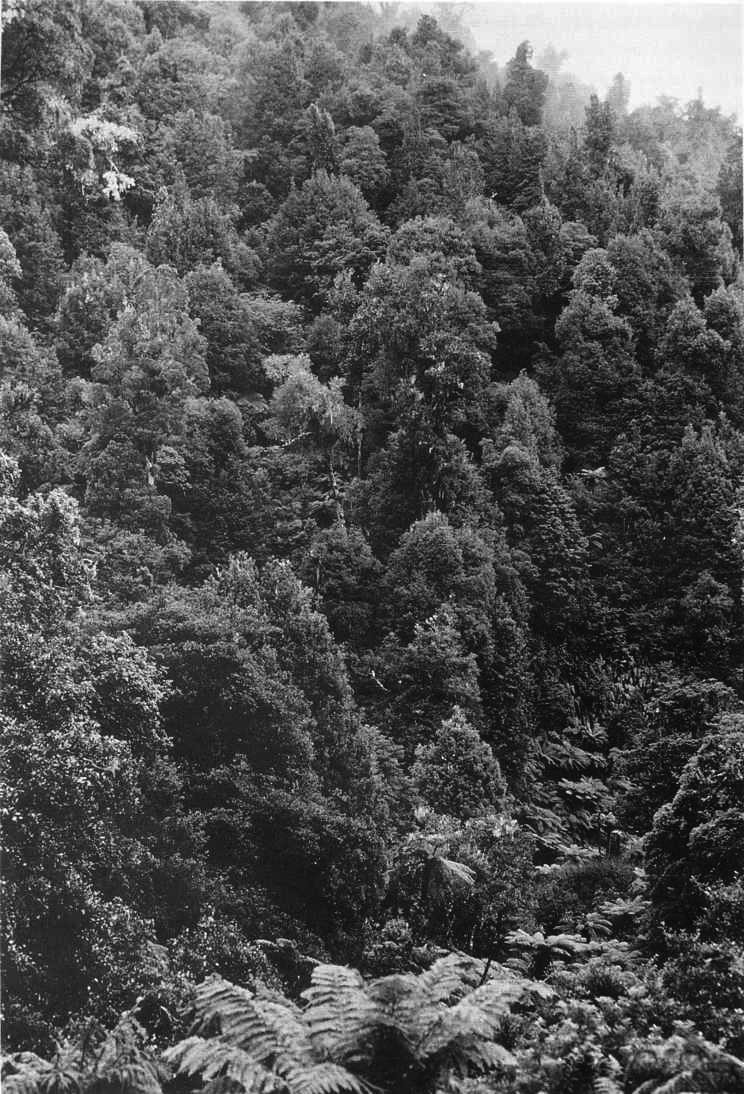
\includegraphics[width=0.66\textwidth]{graphics/fig_006}
	\centering
	\caption[Conifer broadleaf forest, inland Taranaki]{Conifer broadleaf forest.
	Inland Taranaki, west central North Island.
	Photo: J. W. Dawson.}%
	\label{fig:6conifer-broadleaf}%
\end{SCfigure}

A more professional but similar reaction comes in more recent times from a forester from the tropics.\footnote{\cite{brown1960forester}}

\begin{quote}
	I was astonished to find on my arrival that one of the main types of indigenous forest is very similar to Malayan rain forest', far closer to the latter in its structure and appearance than to any type of European forest.
\end{quote}

\afterpage{%
	\begin{figure}[!t]
		% Outer minipage scaled to limit width.
		% Inner minipages scaled so the images have the same height.
		\begin{minipage}[t]{\textwidth}
			\begin{minipage}[t]{(\textwidth-\fgap) * \real{0.545}}% chktex 8
				\centering
				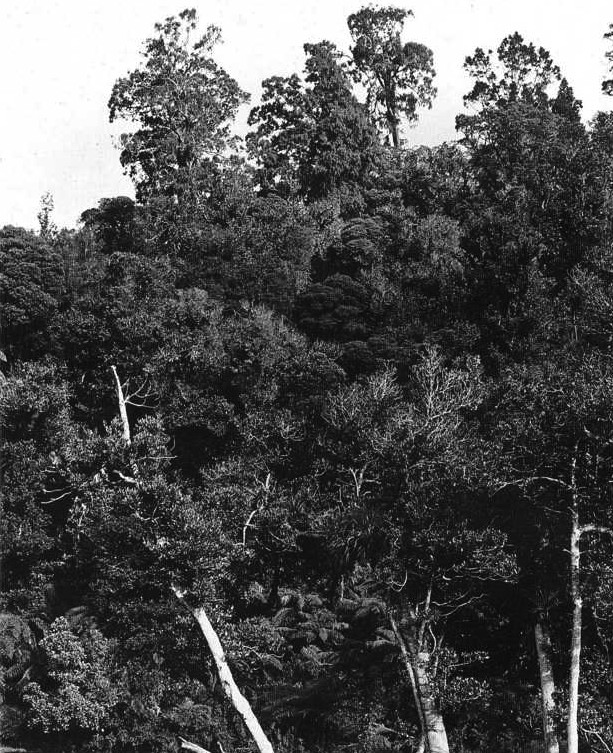
\includegraphics[width=\textwidth]{graphics/fig_007}
				\caption[Conifer broadleaf forest south of Kaitaia]{Conifer broadleaf forest south of Kaitaia, northern North Island.
				The emergent trees on the ridge crest are mostly \IDX{rimu}s (\BotanicRef{Dacrydium cupressinum}[Dacrydium][cupressinum]).
				Photo: B. V. Sneddon.}%
				\label{fig:7conifer}
			\end{minipage}\hspace{\fgap}%
			\begin{minipage}[t]{(\textwidth-\fgap) * \real{0.456}}
				\centering
				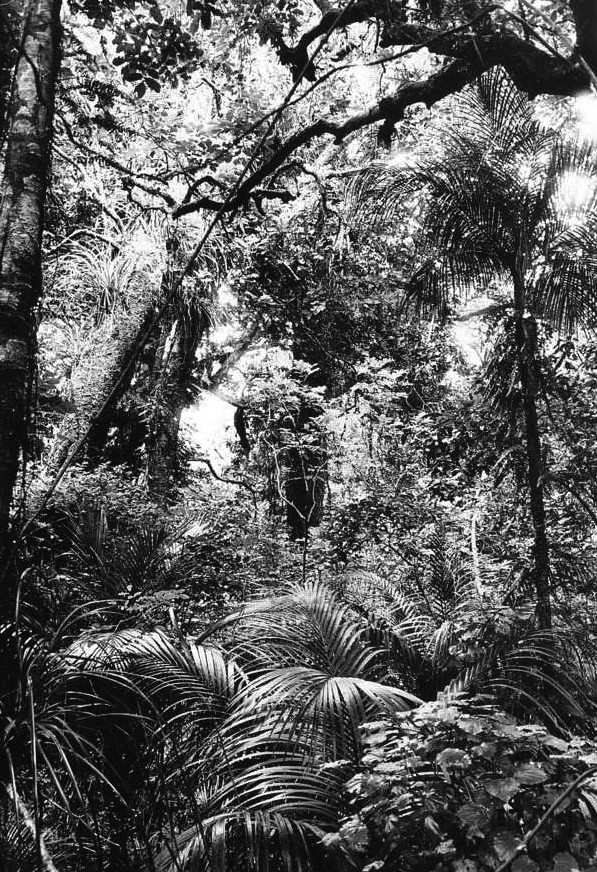
\includegraphics[width=\textwidth]{graphics/fig_008}
				\caption[Interior view of conifer broadleaf forest south of Kaitaia]{Interior view of conifer broadleaf forest south of Kaitaia, northern North Island.
				In the foreground are young plants of the \IDX{nikau palm} (\BotanicRef{Rhopalostylis sapida}[Rhopalostylis][sapida]) and the shrub \IDX{kawakawa} (\BotanicRef{Macropiper excelsum}[Macropiper][excelsum]).
				A larger \IDX{nikau palm} is on the right.
				In the middle distance the shrubs are mostly young plants of the subcanopy tree \IDX{kohekohe} (\BotanicRef{Dysoxylum spectabile}[Dysoxylum][spectabile]).
				The trunks to the left belong to the canopy dominant \IDX{taraire} (\BotanicRef{Beilschmiedia tarairi}[Beilschmiedia][tarairi]) and the large, partly obscured trunk at the centre to the emergent \IDX{northern rata} (\BotanicRef{Metrosideros robusta}[Metrosideros][robusta]).
				Photo: B. V. Sneddon.}%
				\label{fig:8conifer}
			\end{minipage}
		\end{minipage}
	\end{figure}
}

New Zealanders who have grown up with the `bush' do not see it as unusual.
The reason why visitors from comparable latitudes in the northern hemisphere are so taken by surprise is that they expect to find forests similar to those they grew up with: the mid-latitude deciduous forests and the higher latitude coniferous forests with their relatively few species, simple structure and general lack of specialised vines and epiphytes.
Instead they find in the lowlands of New Zealand, particularly at lower northern latitudes, a forest which apparently exhibits all the features they had associated with, and perhaps observed en route, in forests of the tropics.
This being the case, in the following review, consideration of each of the features of mostly free standing plants of New Zealand's conifer broadleaf forest will be preceded by an outline of the comparable features in tropical rain forest.\footnote{\cite{richards1952tropical}}
Forest plants which depend on trees for mechanical support (vines and epiphytes) or nutriment (parasites) will be considered in the next chapter.

\section{Numbers of Species}

Of the major types of world vegetation, tropical rain forest is the most complex in structure and probably the richest in species.
It is found mostly between the tropics of Capricorn and Cancer in regions where rainfall is abundant and evenly spread throughout the year.
The three major regions are west central Africa; south-east Asia to the Pacific; and northern South America and Central America.
These three regions are widely separated geographically and although the forests are vegetationally very similar, each has its own species and in some cases its own genera.
The total numbers of species in these forests are impressive.
Tree species alone are often numbered in the hundreds at many localities, compared with the dozens found in temperate forests.
In most lowland tropical forests the trees are all flowering plants.

In the New Zealand conifer broadleaf forest, tree species are numbered in dozens rather than the hundreds found in tropical rain forest.
Some see this as a major difference precluding any suggestion of a close relationship between the two types of forest.
However, this conclusion may not be justified --- species richness is not the only distinctive feature of tropical rain forest as we shall see.

The conifer broadleaf forest, as the name implies, comprises a mixture of conifers and flowering plants.

\section{Stratification}

Structurally, the tropical rain forest is considered to have five strata; three tree layers, a layer of shrubs and a ground layer of herbaceous plants.
This contrasts with most temperate forests where, at most, three strata are recognised; tree, shrub and ground.

The uppermost layer of very tall trees in the tropical rain forest is often discontinuous and the individual trees are referred to as emergents.
This might be taken to imply that the `emergents' grow through and above the canopy formed by the second tree layer, but studies indicate that many of them are light-demanding species which establish themselves early in a forest's history, grow rapidly, and initially form a continuous layer.
As the lower forest layers close up, the forest floor becomes more shaded, many emergents cease to regenerate, and in time the highest tree stratum becomes discontinuous as old emergents die and are replaced only sporadically in canopy gaps.

In the conifer broadleaf forest five strata can usually be recognised, although they are lower in stature than their tropical equivalents:
\begin{description}
	\item[{(a)}]Emergent trees (\SIrange{30}{40}{\metre}): mostly conifers.
	\item[{(b)}]Canopy trees (\SIrange{20}{25}{\metre}).
	\item[{(c)}]Subcanopy trees (\SIrange{10}{15}{\metre}): including our only native palm, the \IDX{nikau palm} (\BotanicRef{Rhopalostylis sapida}[Rhopalostylis][sapida]) and \BotanicRef{Cyathea} and \BotanicRef{Dicksonia} tree ferns.
	\item[{(d)}]Shrubs and small trees (\SIrange{3}{8}{\metre}).
	\item[{(e)}]Ground plants (\SIrange{0}{1}{\metre}): mostly ferns, but some flowering plants particularly in the north.
\end{description}
\section{Specialised Roots}

A number of tropical trees exhibit structural features which appear strange to the eyes of those from most temperate regions.
Many trees, particularly in swampy situations, develop thin flanges or plank buttresses from the bases of their trunks.
It is suggested that these plank buttresses, which are more or less triangular in form and may extend for several metres up the trunks and out along the roots, confer greater stability on the often shallowly rooted trees.
These plank buttresses are very inconvenient for tree fellers who often find it necessary to construct scaffolding so that the trunk can be sawn through above them.

Other trees increase support for their trunks by forming downward arching prop roots.
This can be seen, perhaps most conspicuously, in \IDX{mangrove} forests.
In swampy situations many trees send up pneumatophores or breathing roots, through which air is taken in and transferred to the root system beneath the swamp.
Pneumatophores are particularly conspicuous in saline coastal swamps inhabited by \IDX{mangrove} forests, but are also found in inland freshwater swamps.
An unusual type of aerial root in tropical forests is the column root, which descends to the ground from horizontal branches, such as in the banyan figs.
Individual banyan trees can sometimes spread out by this means over hectares of ground.

\subsection{Plank Buttresses}

In New Zealand \IDX{pukatea} (\BotanicRef{Laurelia novae-zelandiae}[Laurelia][novae-zelandiae]) often has well defined plank buttresses\figureref{\fullref{fig:9buttresses}}.
Other trees may also have buttresses: \eg\ \IDX{kohekohe} (\BotanicRef{Dysoxylum spectabile}[Dysoxylum][spectabile]), \IDX{kahikatea} (\BotanicRef{Dacrycarpus dacrydioides}[Dacrycarpus][dacrydioides]), and some species of beech (\BotanicRef{Nothofagus}), but these are usually not plank-like.

\begin{figure}[t]
	% Outer minipage scaled to limit width.
	% Inner minipages scaled so the images have the same height.
	\begin{minipage}[t]{\textwidth}
		\begin{minipage}[t]{(\textwidth-\fgap-\fgap) * \real{0.342}}
			\centering
			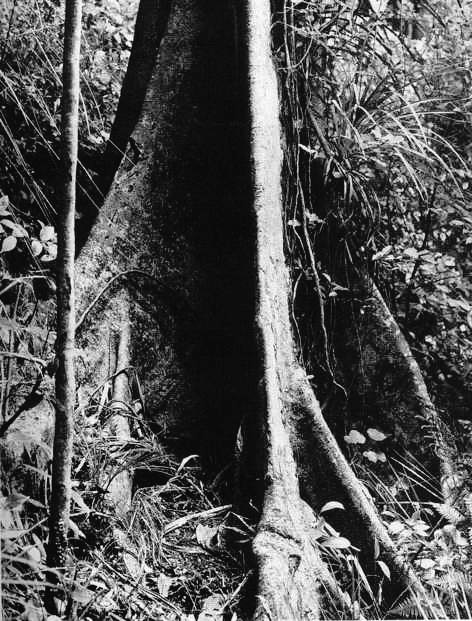
\includegraphics[width=\textwidth]{graphics/fig_009}
			\caption[Plank buttresses of pukatea]{Plank buttresses of \IDX{pukatea} (\BotanicRef{Laurelia novae-zelandiae}[Laurelia][novae-zelandiae]).
			Photo:  F. B. Sampson.}%
			\label{fig:9buttresses}
		\end{minipage}\hspace{\fgap}%
		\begin{minipage}[t]{(\textwidth-\fgap-\fgap) * \real{0.362}}
			\centering
			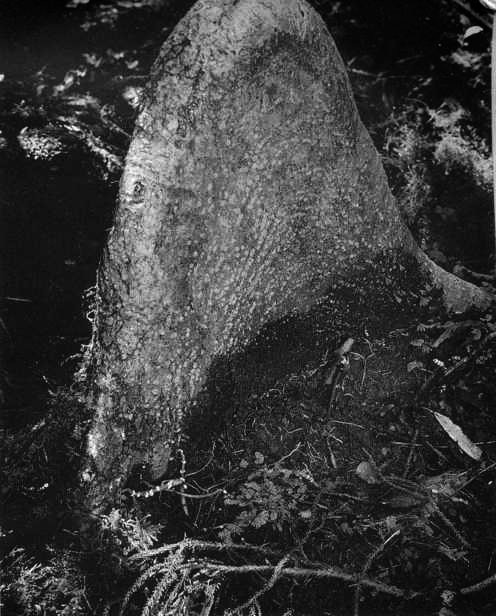
\includegraphics[width=\textwidth]{graphics/fig_010}
			\caption[Pneumatophore of pukatea]{Pneumatophore of \IDX{pukatea} (\BotanicRef{Laurelia novae-zelandiae}[Laurelia][novae-zelandiae]).
			Photo:  M. D. King.}%
			\label{fig:10pukatea}
		\end{minipage}\hspace{\fgap}%
		\begin{minipage}[t]{(\textwidth-\fgap-\fgap) * \real{0.295}}
			\centering
			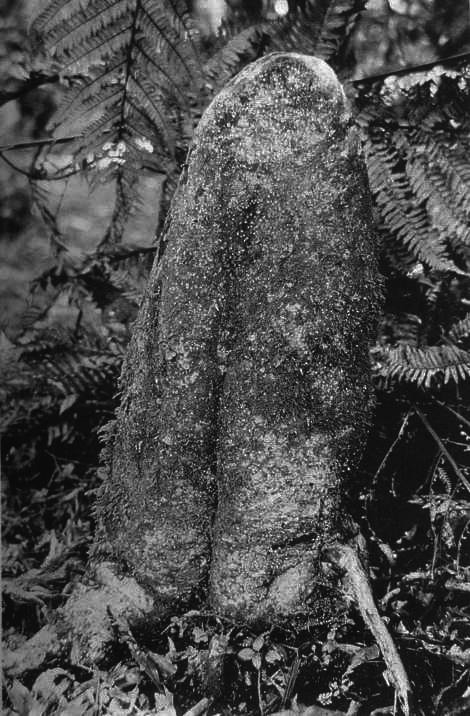
\includegraphics[width=\textwidth]{graphics/fig_011}
			\caption[Pneumatophore of pukatea showing the junction between the two sides of the original loop root]{Pneumatophore of \IDX{pukatea} (\BotanicRef{Laurelia novae-zelandiae}[Laurelia][novae-zelandiae]) showing the junction between the two sides of the original loop root.
			Nga Manu Reserve, Waikanae, southern North Island.
			Photo:  J. E. Casey.}%
			\label{fig:11pukatea}
		\end{minipage}
	\end{minipage}
\end{figure}

\subsection{Pneumatophores}

\IDX{Pukatea}[pukatea], when growing in swamps, also forms large pneumatophores.
These are basically shield-shaped and sometimes several times higher than they are wide\figureref{\fullref{fig:10pukatea}, \fullref{fig:11pukatea}}.
These pneumatophores originate when a root tip arches above the swamp surface and then grows back in again so forming a loop.
Wood is then added mostly on the upper and lower sides of the loop which leads to the eventual shield-shape.
The pneumatophores are covered with mosses and have pustules (lenticels) of loose corky cells, through which air enters the root system.

\begin{figure}[t]
	% Outer minipage scaled to limit width.
	% Inner minipages scaled so the images have the same height.
	\begin{minipage}[t]{\textwidth}
		\begin{minipage}[t]{(\textwidth-\fgap-\fgap) * \real{0.280}}
			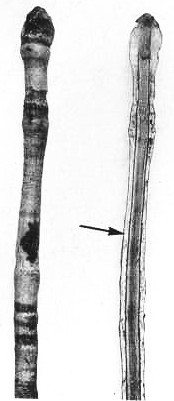
\includegraphics[width=\textwidth]{graphics/fig_012}
			\caption[Pneumatophores of swamp maire]{Pneumatophores of \IDX{swamp maire} (\BotanicRef{Syzygium maire}[Syzygium][maire]).
			The one on the right has been cut in half longitudinally.
			The arrow indicates the white air-filled tissue.
			Photo:  J. E. Casey.}%
			\label{fig:12swampmaire}
		\end{minipage}\hspace{\fgap}%
		\begin{minipage}[t]{(\textwidth-\fgap-\fgap) * \real{0.366}}
			\centering
			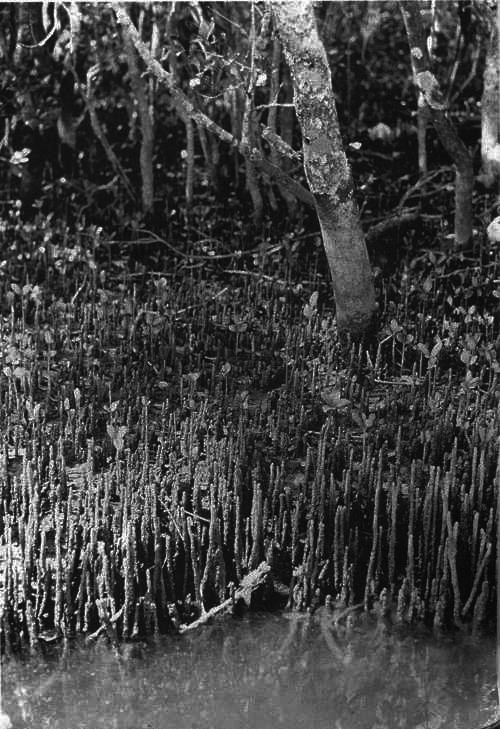
\includegraphics[width=\textwidth]{graphics/fig_013}
			\caption[Pneumatophores of mangrove]{Pneumatophores of \IDX{mangrove} (\BotanicRef{Avicennia resinifera}[Avicennia][resinifera], \IDX{manawa}).
			Near Kaeo, northern North Island.
			Photo:  J. W. Dawson.}%
			\label{fig:13mangrove}
		\end{minipage}\hspace{\fgap}%
		\begin{minipage}[t]{(\textwidth-\fgap-\fgap) * \real{0.354}}
			\centering
			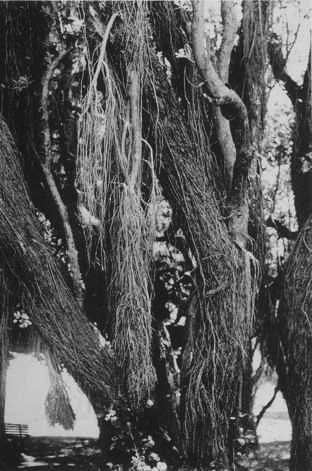
\includegraphics[width=\textwidth]{graphics/fig_015}
			\caption[Aerial roots of pohutukawa]{Aerial roots of \IDX{pohutukawa} (\BotanicRef{Metrosideros excelsa}[Metrosideros][excelsa]).
			Photo:  J. W. Dawson.}%
			\label{fig:15pohutakawa}
		\end{minipage}
	\end{minipage}
\end{figure}

\IDX{Swamp maire}[swamp maire] (\BotanicRef{Syzygium maire}[Syzygium][maire], \IDX{maire tawake}, \IDX{waiwaka}) is often associated with \IDX{pukatea} in swamp forests and it too forms specialised pneumatophores.
In this case, however, they are not woody loops, but smaller, finger-like and rather spongy root tips several centimetres long.
They are orangey-brown in colour and often branch near the base to form coral-like clusters.
A longitudinal section through such a `peg root' reveals a white outer cylinder of air-filled tissue\figureref{\fullref{fig:12swampmaire}}.

In the same swamps, \IDX{kiekie} (\BotanicRef{Freycinetia baueriana var.\ banksii}[Freycinetia][baueriana var.\ banksii]) often sprawls on the forest floor as well as climbing up tree trunks.
In the former situation it forms what may be pneumatophores of an unusual type.
They are slender and finger-like, and have a succession of tyre-like rings of white aeration tissue.

Finally the pneumatophores which catch the eye of many people in the Auckland region are those formed by the \IDX{mangrove}s.
These too are finger-like and project above the mud surface at low tide\figureref{\fullref{fig:13mangrove}}.

\subsection{Prop Roots}

\begin{SCfigure}[0.5][t]
	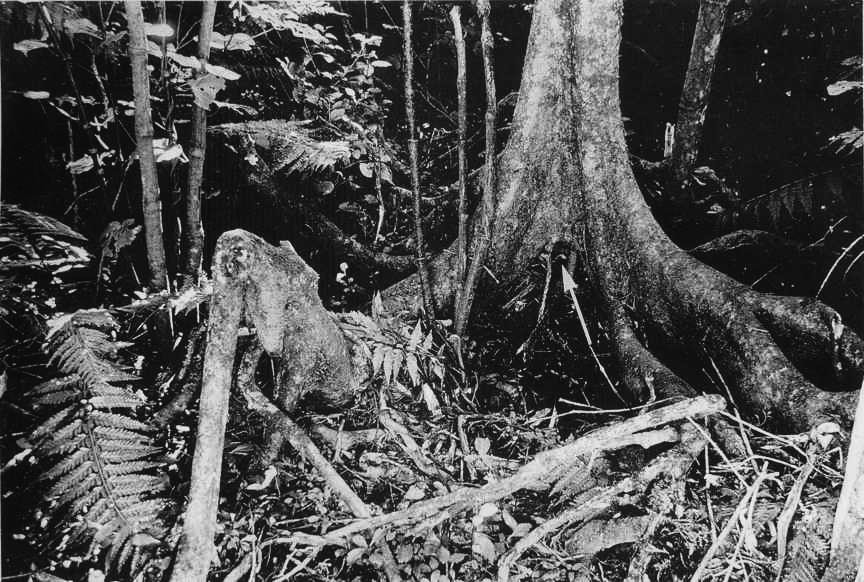
\includegraphics[width=0.66\textwidth]{graphics/fig_014}
	\centering
	\caption[Roots of swamp maire]{Roots of \IDX{swamp maire} (\BotanicRef{Syzygium maire}[Syzygium][maire], \IDX{maire tawake}, \IDX{waiwaka}).
	The arrow indicates the space below the base of the trunk where the primary root failed to develop.
	Nga Manu Reserve, Waikanae, near Wellington, southern North Island.
	Photo:  J. E. Casey.}%
	\label{fig:14swampmaire}
\end{SCfigure}

In the \IDX{swamp maire} the primary root in young plants often atrophies or becomes weak, and prop roots develop from the base of the trunk to provide the root system of the adult tree.
In young trees the space between the base of the trunk and the ground is readily observable\figureref{\fullref{fig:14swampmaire}}.

The \IDX{nikau palm} may also produce a fringe of slender prop roots a little above ground level.

\subsection{Column Roots}

\IDX{Pohutukawa}[pohutukawa] (\BotanicRef{Metrosideros excelsa}[Metrosideros][excelsa]) forms aerial roots very readily, which run down the trunk to the ground.
Sometimes it forms column roots from more-or-less horizontal branches.
Except where the trees have a semi-sprawling habit on coastal cliffs, these roots often do not reach the ground, but branch profusely at the lower end to give a straw broom effect\figureref{\fullref{fig:15pohutakawa}}.
Similar roots can be observed in some tropical figs (\BotanicRef{Ficus}).

\section{Cauliflory}

A strange habit of some tropical trees is the production of flowers directly on the trunks and/or branches, a phenomenon known as cauliflory.
The most notable New Zealand example of this is \IDX{kohekohe} (\BotanicRef{Dysoxylum spectabile}[Dysoxylum][spectabile]) where the sprays of orange-blossom-like flowers may be produced directly on the trunks\figureref{\fullref{fig:16infloresence}} as well as on the major branches.

The flowers of the \IDX{tree fuchsia} (\BotanicRef{Fuchsia excorticata}[Fuchsia][excorticata], \IDX{kotukutuku}) are mostly produced towards the ends of woody branches, but sometimes appear directly on the trunk.

Two rare species on the Three Kings Islands, \IDX{akapukaea} (\BotanicRef{Tecomanthe speciosa}[Tecomanthe][speciosa]) and \IDX{Three Kings kaikomako} (\BotanicRef{Pennantia baylisiana}[Pennantia][baylisiana]) are also cauliflorous.

In the species of \BotanicRef{Myrsine}, \BotanicRef{Melicytus}\figureref{\fullref{fig:17mahoe}} the liane \IDX{white rata} (\BotanicRef{Metrosideros diffusa}[Metrosideros][diffusa]) and \IDX{Parkinson's rata}[rata!Parkinson's] (\BotanicRef{Metrosideros parkinsonii}[Metrosideros][parkinsonii]), the flowers arise on woody twigs towards the tips of branches, a less extreme condition often known as ramiflory.

\begin{figure}[t]
	% Outer minipage scaled to limit width.
	% Inner minipages scaled so the images have the same height.
	\begin{minipage}[t]{\textwidth}
		\begin{minipage}[t]{(\textwidth-\fgap) * \real{0.622}}
			\centering
			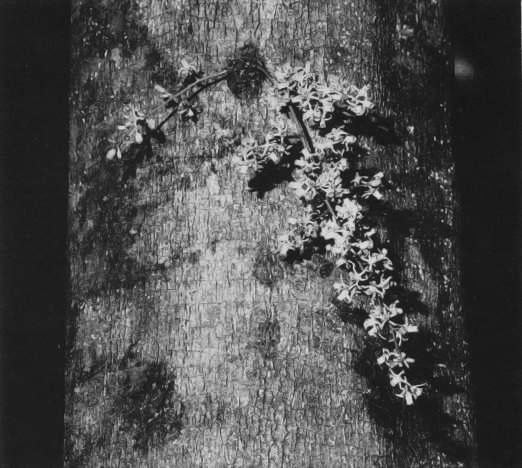
\includegraphics[width=\textwidth]{graphics/fig_016}
			\caption[Inflorescence arising directly from the trunk of kohekohe]{Inflorescence arising directly from the trunk of \IDX{kohekohe} (\BotanicRef{Dysoxylum spectabile}[Dysoxylum][spectabile]).
			Photo:  M. D. King.}%
			\label{fig:16infloresence}
		\end{minipage}\hspace{\fgap}%
		\begin{minipage}[t]{(\textwidth-\fgap) * \real{0.378}}
			\centering
			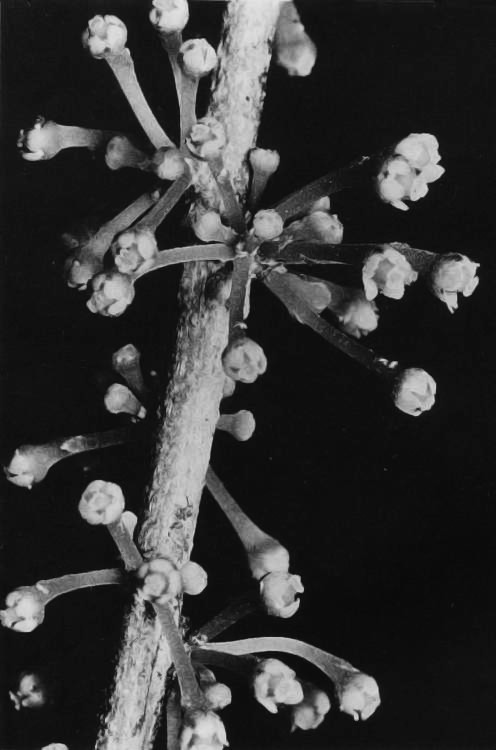
\includegraphics[width=\textwidth]{graphics/fig_017}
			\caption[Ramiflory.
			Female flowers of mahoe]{Ramiflory.
			Female flowers of \IDX{mahoe} (\BotanicRef{Melicytus ramiflorus}[Melicytus][ramiflorus]) borne on woody twigs.
			Photo:  M. D. King.}%
			\label{fig:17mahoe}
		\end{minipage}
	\end{minipage}
\end{figure}

\section{Leaf Features}

The leaves of plants of moist tropical forests are evergreen, generally larger than those of temperate forests and are often leathery and smooth-margined.
Average leaf size decreases with increasing height above the ground and some of the trees have distinct juvenile forms with leaves much larger and/or more compound than those of the adults.
In some cases there are narrow prolongations from the ends of the leaves known as `drip tips', thought by some to enable rapid drying of leaves after rain.

Pulvini or elastic swellings at one or both ends of the leaf stalk or petiole are a common feature of tropical forest plants.
It has been suggested that bending movements at these pulvini enable the leaf to maintain the best orientation to the light.

\subsection{Leaf size}

The average leaf size is considerably less in the New Zealand conifer broadleaf than in tropical rain forest.
This can be demonstrated by comparing the species of a far northern New Zealand forest with a Philippines forest in terms of a now widely accepted leaf size classification.

\begin{tabular}{ l c }
	\toprule
	\emph{Philippines Forest}\footnote{\cite{richards1952tropical}}\\
	Species with macrophylls (leaves \SIrange{18}{60}{\centi\metre} long\footnote{Based on leaves about twice as long as they are wide}) & 10\%\\
	Species with mesophylls (leaves \SIrange{6}{18}{\centi\metre} long) & 86\%\\
	Species with microphylls (leaves \SIrange{2}{6}{\centi\metre} long) & 4\%\\
	\emph{New Zealand Forest}\footnote{\cite{dawson1969lowland}}\\
	Species with macrophylls & 1\%\\
	Species with mesophylls & 25\%\\
	Species with microphylls & 68\%\\
	Species with nanophylls (leaves \SIrange{1}{2}{\centi\metre} long) & 6\%\\
	\bottomrule
\end{tabular}

The smaller leaf sizes in New Zealand probably correlate with lower temperatures.\footnote{\cite{dawson1986floristic}}

\subsection{Teeth, Pulvini and Drip Tips}

The proportion of woody dicotyledon species in the conifer broadleaf forest with smooth-margined leaves or leaflets is lower than that of tropical forests: about 56 per cent compared with 80 per cent recorded, in a Nigerian forest.\footnote{\cite{richards1952tropical}}
Godley\footnote{\cite{godley1985paths}} has observed that some New Zealand trees have much more prominent teeth on the leaves of young plants than on those of adults; for example \IDX{wineberry} (\BotanicRef{Aristotelia serrata}[Aristotelia][serrata]) and \IDX{ngaio} (\BotanicRef{Myoporum laetum}[Myoporum][laetum]).
In other cases, some trees with smooth-margined adult leaves or leaflets have juvenile leaves with toothed or lobed margins; for example \IDX{puriri} (\BotanicRef{Vitex lucens}[Vitex][lucens]), \IDX{titoki} (\BotanicRef{Alectryon excelsus}[Alectryon][excelsus]), \IDX{kohekohe} (\BotanicRef{Dysoxylum spectabile}[Dysoxylum][spectabile]) and several species of \BotanicRef{Hebe}.

Pulvini also are not common.
The species of \IDX{maire} (\BotanicRef{Nestegis}) have dark-coloured pulvini at the petiole bases and \IDX{kohekohe} (\BotanicRef{Dysoxylum spectabile}[Dysoxylum][spectabile]), \IDX{titoki} (\BotanicRef{Alectryon excelsus}[Alectryon][excelsus]) and king fern (\BotanicRef{Marattia salicina}[Marattia][salicina]) have them at the bases of the leaflet petioles.
\IDX{Hinau}[hinau] (\BotanicRef{Elaeocarpus dentatus}[Elaeocarpus][dentatus]) is an interesting case.
The adult leaves do not have pulvini, but on juvenile leaves they can be observed at each end of the petioles.
The larger-leaved tropical species of \BotanicRef{Elaeocarpus} have prominent pulvini in the same position on adult leaves.

Drip tips are neither strongly developed nor very common in the New Zealand forest.
In fact the most that can be said is that ten or so species tend to have slightly to moderately drawn out leaf tips especially when growing under sheltered, shady conditions.
Perhaps both drip tips and pulvini were better developed in the ancestors of our present trees.

\subsection[Juvenile Forms]{Juvenile Forms\thinspace\footnote{\cite{godley1985paths}}\footnote{\cite{philipson1964habit}}}

Often very distinct juvenile and adult forms are a noticeable and, to those learning to identify native plants, a tiresome feature of the New Zealand flora.
In the conifer broadleaf forest, some of the juveniles contrast with those of the tropics in that they are very freely branched with leaves much smaller than on the adults.
These will be considered in Chapter~\ref{ch:shrubs} \nameref{ch:shrubs} as part of the wider question of the small-leaved, freely branched or `divaricating' shrubs, so prevalent in New Zealand.

The remaining rain forest species under this heading have juvenile leaves which are larger or longer or more compound or more dissected than those of the adults.

\IDX{Raukawa}[raukawa] (\BotanicRef{Pseudopanax edgerleyii}[Pseudopanax][edgerleyii]) has palmately compound juvenile leaves with up to five deeply lobed leaflets.
The adult leaves are simple and smooth-margined.

One variety of \IDX{haumakoroa} (\BotanicRef{Pseudopanax simplex}[Pseudopanax][simplex]) has juvenile leaves very similar to those of \IDX{raukawa} (\BotanicRef{Pseudopanax edgerleyii}[Pseudopanax][edgerleyii]) and simple, toothed adult leaves\figureref{\fullref{fig:18pseudopanax}}.

\begin{figure}[!b]
	% Outer minipage scaled to limit width.
	% Inner minipages scaled so the images have the same height.
	\begin{minipage}[t]{\textwidth}
		\begin{minipage}[t]{(\textwidth-\fgap) * \real{0.526}}
			\centering
			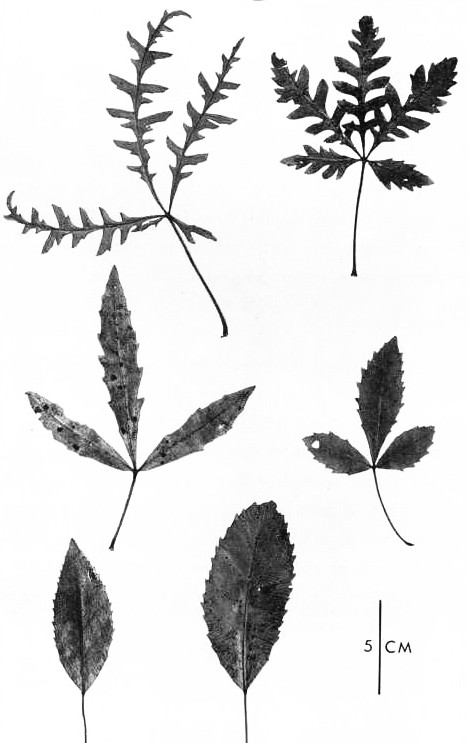
\includegraphics[width=\textwidth]{graphics/fig_018}
			\caption[Juvenile and adult leaves of \emph{Pseudopanax simplex var.\ simplex}]{Juvenile and adult leaves of \IDX{haumakoroa} (\BotanicRef{Pseudopanax simplex var.\ simplex}[Pseudopanax][simplex var.\ simplex]).
			Dissected compound juvenile leaves above; serrate, compound semi-juvenile leaves centre; simple, serrate adult leaves below.
			Photo: J. E. Casey.}%
			\label{fig:18pseudopanax}
		\end{minipage}\hspace{\fgap}%
		\begin{minipage}[t]{(\textwidth-\fgap) * \real{0.474}}
			\centering
			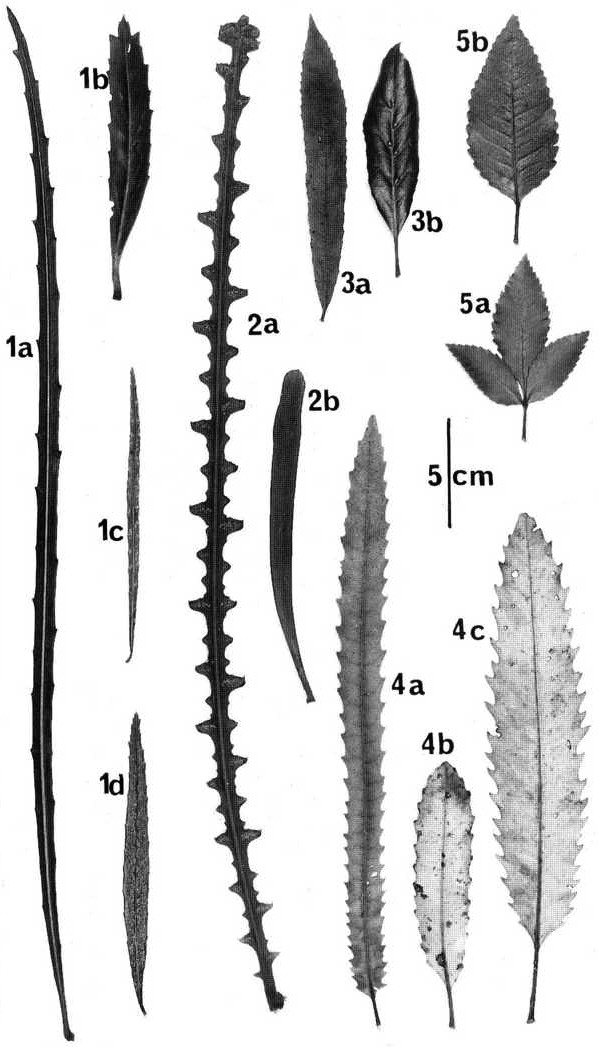
\includegraphics[width=\textwidth]{graphics/fig_019}
			\caption[Juvenile and adult leaves]{Juvenile and adult leaves.
			\IDX{Lancewood}[lancewood] (\BotanicRef{Pseudopanax crassifolius}[Pseudopanax][crassifolius]):
			1a, juvenile leaf;
			1b, adult leaf;
			1c, 1d,brown, mottled leaves from a seedling.
			\IDX{Fierce lancewood}[fierce lancewood] (\BotanicRef{Pseudopanax ferox}[Pseudopanax][ferox]):
			2a, coarsely toothed juvenile leaf;
			2b, adult leaf.
			\IDX{Hinau}[hinau] (\BotanicRef{Elaeocarpus dentatus}[Elaeocarpus][dentatus]):
			3a, juvenile leaf;
			3b, adult leaf (note domatia).
			\IDX{Rewarewa}[rewarewa] (\BotanicRef{Knightia excelsa}[Knightia][excelsa]):
			4a, juvenile leaf;
			4b, c, adult leaves.
			\IDX{Kamahi}[kamahi] (\BotanicRef{Weinmannia racemosa}[Weinmannia][racemosa]):
			5a, trifoliolate juvenile leaf;
			5b, simple adult leaf.
			Photo  J. E. Casey.}%
			\label{fig:19leaves}
		\end{minipage}
	\end{minipage}
\end{figure}

\IDX{Pate}[pate] (\BotanicRef{Schefflera digitata}[Schefflera][digitata]) is unusual in that juvenile leaves are only found on some plants in the northern half of the North Island.
These leaves are palmately compound and similar in size to those of the adults, but the leaflets are deeply lobed rather than just toothed.

In three tree species, all belonging to the family Cunoniaceae, the leaves are basically pinnately compound.
In \IDX{makamaka} (\BotanicRef{Ackama rosifolia}[Ackama][rosifolia]) the juveniles have six to ten pairs of leaflets, the adults three to five.
In \IDX{towai} (\BotanicRef{Weinmannia silvicola}[Weinmannia][silvicola]) the trend is from five to one pairs of leaflets; in \IDX{kamahi} (\BotanicRef{Weinmannia racemosa}[Weinmannia][racemosa]) from one or two pairs of leaflets to simple leaves\figureref{\fullref{fig:19leaves}}.

In all cases where the juvenile leaves are compound and the adult leaves simple, the latter have a distinct joint at the end of the petiole as an indication of their compound derivation.

Only a few New Zealand species have juvenile leaves which are broad and much larger than the adults: \IDX{wineberry} (\BotanicRef{Aristotelia serrata}[Aristotelia][serrata]), \BotanicRef{Nestegis apetala}[Nestegis][apetala] and \IDX{Chatham Island karamu} (\BotanicRef{Coprosma chathamica}[Coprosma][chathamica]).
In several species of \BotanicRef{Dracophyllum}, where all the leaves are long and narrow, the juvenile leaves are much larger than the adults.
In species of other genera the juvenile leaves are themselves very small but they are still larger than the adult leaves, which are reduced to scales, as in several species of `whipcord' \BotanicRef{Hebe}, \IDX{coral sea shrub}0(\BotanicRef{Helichrysum coralloides}[Helichrysum][coralloides]) and a group of conifers formerly included in \BotanicRef{Dacrydium}; \IDX{silver pine} (\BotanicRef{Lagarostrobos colensoi}[Lagarostrobos][colensoi]), \IDX{yellow silver pine} (\BotanicRef{Lepidothamnus intermedius}[Lepidothamnus][intermedius]), \IDX{bog pine} (\BotanicRef{Halocarpus bidwillii}[Halocarpus][bidwillii]), \IDX{pink pine} (\BotanicRef{Halocarpus biformis}[Halocarpus][biformis]) and \IDX{manoao} (\BotanicRef{Halocarpus kirkii}[Halocarpus][kirkii]).
In the latter cases there is an abrupt change from juvenile to adult leaves.
Two other conifers with scale-leaved adults are our only \BotanicRef{Dacrydium} --- \IDX{rimu} (\BotanicRef{Dacrydium cupressinum}[Dacrydium][cupressinum]) and \IDX{kahikatea} (\BotanicRef{Dacrycarpus dacrydioides}[Dacrycarpus][dacrydioides])\figureref{\fullref{fig:21rimu}, \fullref{fig:22kahikatea}}.
In both of these the juvenile leaves are small and needle-like.
The juveniles of \IDX{rimu} are notable for their attractive weeping habit.

\begin{figure}[t]
	% Outer minipage scaled to limit width.
	% Inner minipages scaled so the images have the same height.
	\begin{minipage}[t]{\textwidth}
		\begin{minipage}[t]{(\textwidth-\fgap) * \real{0.503}}
			\centering
			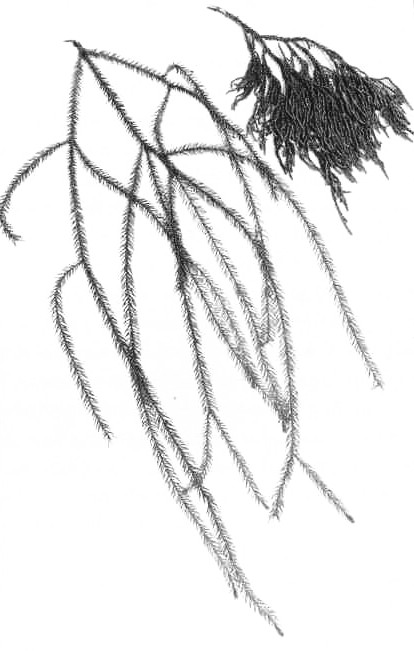
\includegraphics[width=\textwidth]{graphics/fig_021}
			\caption[Rimu foliage]{Juvenile (below) and adult foliage of \IDX{rimu} (\BotanicRef{Dacrydium cupressinum}[Dacrydium][cupressinum]).
			Photo: J. E. Casey.}%
			\label{fig:21rimu}
		\end{minipage}\hspace{\fgap}%
		\begin{minipage}[t]{(\textwidth-\fgap) * \real{0.497}}
			\centering
			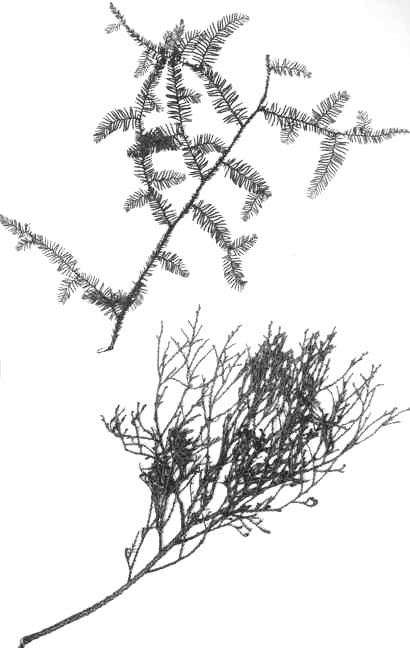
\includegraphics[width=\textwidth]{graphics/fig_022}
			\caption[Kahikatea foliage]{Juvenile (above) and adult foliage of \IDX{kahikatea} (\BotanicRef{Dacrycarpus dacrydioides}[Dacrycarpus][dacrydioides]).
			Photo: J. E. Casey.}%
			\label{fig:22kahikatea}
		\end{minipage}
	\end{minipage}
\end{figure}

In most of the species that follow, juvenile leaves are as narrow as the adult or narrower, but may have a larger area by virtue of their greater length.
This is not a pattern familiar in the tropics, although on Mauritius and Reunion Islands in the Indian Ocean there is a partly comparable pattern --- one species each of 24 genera has juvenile leaves which are much narrower than the adult leaves and also much smaller in area.\footnote{\cite{friedmann1976observations}}

\IDX{Lancewood}[lancewood] (\BotanicRef{Pseudopanax crassifolius}[Pseudopanax][crassifolius])\figureref{\fullref{fig:19leaves}, \fullref{fig:20lancewood}} is the best known of our trees with a juvenile form.\footnote{\cite{laing1906plants}}
The juvenile leaves are several times longer than those of the adult and a little narrower.
They hang down in a distinctive cluster from the tip of the slender stem, which does not branch until it attains a height of \SIrange{4}{5}{\metre} after 15 or more years.
The stem is then able to branch into a dense and rounded crown with short, broad, upwardly directed adult leaves.
The related but less common \IDX{fierce lancewood} (\BotanicRef{Pseudopanax ferox}[Pseudopanax][ferox]) is very similar, but the juvenile leaves have very coarse irregularly-shaped teeth.
\IDX{Lancewood}[lancewood] also has a distinct seedling form in which the leaves are very variable in shape, size and degree of dissection.
\IDX{Rewarewa}[rewarewa] (\BotanicRef{Knightia excelsa}[Knightia][excelsa]) and \IDX{hinau} (\BotanicRef{Elaeocarpus dentatus}[Elaeocarpus][dentatus]) with their long narrow juvenile leaves have a juvenile-adult pattern similar to \IDX{lancewood}, but branching is initiated at an earlier stage.
The juvenile leaves of \IDX{hinau} are soft, widest near the tip and have obscure teeth; those of \IDX{rewarewa} are stiff, of even width and have coarse teeth.
As mentioned earlier, the juvenile leaves of \IDX{hinau} may have pulvini, which the adult does not, but the adult leaves have pouch-like cavities or domatia\figureref{\fullref{fig:23hinau}},\footnote{\cite{sampson1965domatia}} where the secondary veins meet the midrib on the undersides.

\begin{figure}[!t]
	% Outer minipage scaled to limit width.
	% Inner minipages scaled so the images have the same height.
	\begin{minipage}[t]{\textwidth}
		\begin{minipage}[t]{(\textwidth-\fgap) * \real{0.491}}
			\centering
			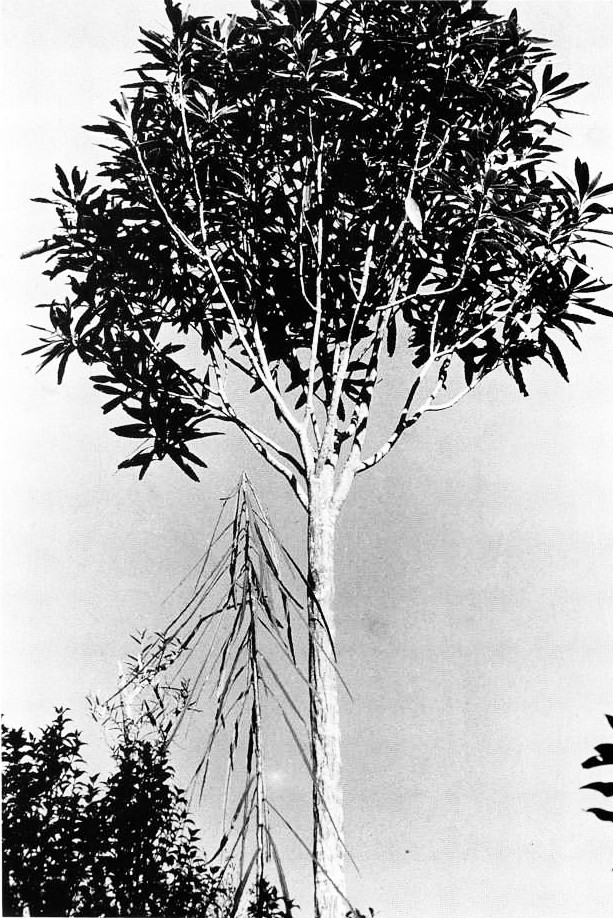
\includegraphics[width=\textwidth]{graphics/fig_020}
			\caption[Adult lancewood]{Adult \IDX{lancewood} (\BotanicRef{Pseudopanax crassifolius}[Pseudopanax][crassifolius]), with a basal shoot of completely juvenile form to the left.
			Nga Manu Reserve, Waikanae, southern North Island.
			Photo: J. E. Casey.}%
			\label{fig:20lancewood}
		\end{minipage}\hspace{\fgap}%
		\begin{minipage}[t]{(\textwidth-\fgap) * \real{0.509}}
			\centering
			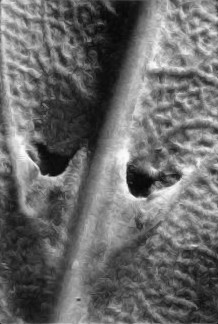
\includegraphics[width=\textwidth]{graphics/fig_023}
			\caption[Domatia of the adult leaves of hinau]{Domatia of the adult leaves of \IDX{hinau} (\BotanicRef{Elaeocarpus dentatus}[Elaeocarpus][dentatus]).
			The pouch-like domatia form at the junctions of the secondary veins and the midrib.
			Photo: M. D. King.}%
			\label{fig:23hinau}
		\end{minipage}
	\end{minipage}
\end{figure}

Three of the four species of \BotanicRef{Nestegis} or `native olives' have narrow adult leaves.
In the case of two species, \IDX{black maire} (\BotanicRef{Nestegis cunninghamii}[Nestegis][cunninghamii]) and \IDX{white maire} (\BotanicRef{Nestegis lanceolata}[Nestegis][lanceolata]), the juveniles are much narrower than the adults, but as they are also often longer they may have about the same area as the adult leaves or somewhat less.
The last species,\IDX{narrow-leaved maire} (\BotanicRef{Nestegis montana}[Nestegis][montana]), has adult and juvenile leaves which are almost equally narrow, but the juveniles, being longer, are greater in area than the adults.

Trees with distinct juveniles may exhibit a curious phenomenon whereby fully adult specimens give rise to shoots near the ground which bear leaves of juvenile form\figureref{\fullref{fig:20lancewood}}.
These are termed reversion shoots and they derive from dormant buds formed during the juvenile phase of the tree and so are `programmed' to be juvenile.
\IDX{Pokaka}[pokaka] (\BotanicRef{Elaeocarpus hookerianus}[Elaeocarpus][hookerianus]) may be an exception, as reversion shoots can occur \SI{10}{\metre} or more above the ground; well above the height of the juvenile stage.

\subsection{The Deciduous Habit}

In north temperate forests many trees and shrubs are leafless during the winter, and in tropical forests some species, growing in areas where there is a distinct dry season, may be leafless during the unfavourable period.
In the New Zealand rain forest, which grows in parts of the country where there is no well-marked dry season and winters are relatively mild, the deciduous habit is uncommon.\footnote{\cite{bussell1968growth}}\footnote{\cite{bussell1968effects}}\footnote{\cite{russel1936mechanism}} The following New Zealand conifer broadleaf forest species are or may be leafless during winter: \IDX{wineberry} (\BotanicRef{Aristotelia serrata}[Aristotelia][serrata])\BotanicRef{Fuchsia excorticata}[Fuchsia][excorticata], the vines \IDX{pohuehue} (\BotanicRef{Muehlenbeckia australis}[Muehlenbeckia][australis]) and \IDX{scrub pohuehue} (\BotanicRef{Muehlenbeckia complexa}[Muehlenbeckia][complexa]), and \IDX{ribbonwood} (\BotanicRef{Plagianthus regius}[Plagianthus][regius]).
Some forms of \IDX{kowhai} (\BotanicRef{Sophora microphylla}[Sophora][microphylla]) lose their leaves in the spring before flowering.
However, with at least \BotanicRef{Fuchsia} and \BotanicRef{Aristotelia}, leaf fall is more related to temperature than to declining day length, which is the triggering factor for most northern temperate deciduous trees.
Both species may be evergreen in milder latitudes.\footnote{\cite{cockayne1928vegetation}}

\section{Bud Protection}

Unlike many trees of temperate climates, where the immature leaves at the branch tips are protected during the winter by dry overlapping scales, the buds of many tropical trees of moist climates are not protected in this way.
This is understandable as they are not subject to an unfavourable season.
Nevertheless the delicate immature leaves are at some risk of drying out and they may be protected by a layer of hairs or by mucilaginous or resinous secretions.
The petiole bases of mature leaves adjacent to a bud may also afford some protection by partly enclosing it with or without the assistance of paired appendages known as stipules.

In this respect the woody flowering plants of the New Zealand conifer broadleaf forest seem comparable to those of the tropics.
Of 45 genera only 3 have numerous, relatively large bud scales --- \BotanicRef{Pittosporum}\figureref{\fullref{fig:24tarata}}, \BotanicRef{Aristotelia} and the tree species of \BotanicRef{Metrosideros}.
In the beech forest (see Chapter~\ref{ch:beechforests} \nameref{ch:beechforests}) the species of \BotanicRef{Nothofagus} also have many overlapping bud scales.

Nineteen genera have no bud protective structures at all although the immature leaves are often hairy\figureref{\fullref{fig:25rewarewa}}.
Admittedly, genera in this group with strong tropical affinities, for example \BotanicRef{Dysoxylum}, \BotanicRef{Vitex}, \BotanicRef{Beilschmiedia}, \BotanicRef{Litsea}, are represented by only one or two species in New Zealand.

\begin{figure}[t]
	% Outer minipage scaled to limit width.
	% Inner minipages scaled so the images have the same height.
	\begin{minipage}[t]{\textwidth}
		\begin{minipage}[t]{(\textwidth-\fgap) * \real{0.677}}
			\centering
			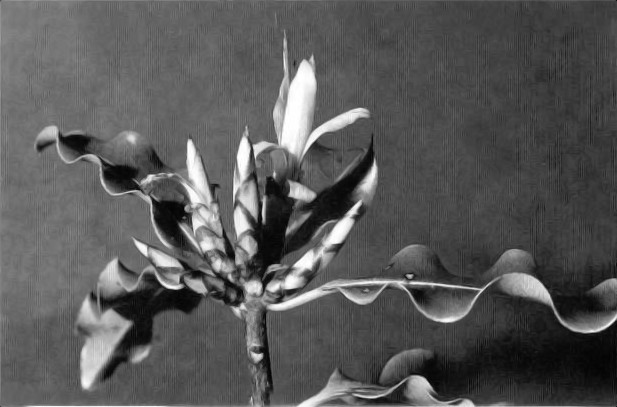
\includegraphics[width=\textwidth]{graphics/fig_024}
			\caption[Tarata or lemonwood]{\IDX{Tarata} or lemonwood (\BotanicRef{Pittosporum eugenioides}[Pittosporum][eugenioides]). Overwintering buds with overlapping bud scales. Photo: M. D. King.}%
			\label{fig:24tarata}
		\end{minipage}\hspace{\fgap}%
		\begin{minipage}[t]{(\textwidth-\fgap) * \real{0.323}}
			\centering
			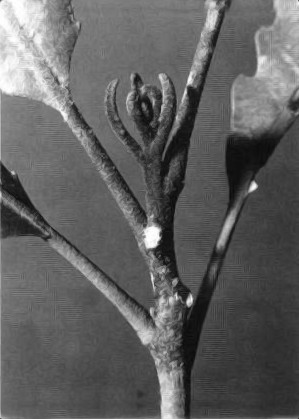
\includegraphics[width=\textwidth]{graphics/fig_025}
			\caption[Rewarewa leaves]{Rewarewa (\BotanicRef{Knightia excelsa}[Knightia][excelsa]).
			Very young leaves with a furry pubescence, but otherwise unprotected.
			Photo: M. D. King.}%
			\label{fig:25rewarewa}
		\end{minipage}
	\end{minipage}
\end{figure}

The remaining genera afford their immature leaves partial or complete protection with a few small scales or with the stipules or sheathing bases of adjacent mature or developing leaves.
Some also form protective secretions such as mucilage in \BotanicRef{Coprosma} and a varnish-like material in some species of \BotanicRef{Pseudopanax}.
